%%%%%%%%%%%%%%%%%%%%%%%%%%%%%%%%%%%%%%%%%
% Short Sectioned Assignment
% LaTeX Template
% Version 1.0 (5/5/12)
%
% This template has been downloaded from:
% http://www.LaTeXTemplates.com
%
% Original author:
% Frits Wenneker (http://www.howtotex.com)
%
% License:
% CC BY-NC-SA 3.0 (http://creativecommons.org/licenses/by-nc-sa/3.0/)
%
%%%%%%%%%%%%%%%%%%%%%%%%%%%%%%%%%%%%%%%%%

%----------------------------------------------------------------------------------------
%	PACKAGES AND OTHER DOCUMENT CONFIGURATIONS
%----------------------------------------------------------------------------------------

\documentclass[paper=a4, fontsize=11pt]{scrartcl} % A4 paper and 11pt font size

\usepackage[T1]{fontenc} % Use 8-bit encoding that has 256 glyphs
\usepackage{fourier} % Use the Adobe Utopia font for the document - comment this line to return to the LaTeX default
\usepackage[spanish]{babel} % English language/hyphenation
\selectlanguage{spanish}
\usepackage[utf8]{inputenc}
\usepackage{amsmath,amsfonts,amsthm} % Math packages
\usepackage{graphicx}

\usepackage{sectsty} % Allows customizing section commands
\allsectionsfont{\centering \normalfont\scshape} % Make all sections centered, the default font and small caps

\usepackage{fancyhdr} % Custom headers and footers
\pagestyle{fancyplain} % Makes all pages in the document conform to the custom headers and footers
\date{}
\fancyhead{} % No page header - if you want one, create it in the same way as the footers below
\fancyfoot[L]{} % Empty left footer
\fancyfoot[C]{} % Empty center footer
\fancyfoot[R]{\thepage} % Page numbering for right footer
\renewcommand{\headrulewidth}{0pt} % Remove header underlines
\renewcommand{\footrulewidth}{0pt} % Remove footer underlines
\setlength{\headheight}{5.6pt} % Customize the height of the header

\numberwithin{equation}{section} % Number equations within sections (i.e. 1.1, 1.2, 2.1, 2.2 instead of 1, 2, 3, 4)
\numberwithin{figure}{section} % Number figures within sections (i.e. 1.1, 1.2, 2.1, 2.2 instead of 1, 2, 3, 4)
\numberwithin{table}{section} % Number tables within sections (i.e. 1.1, 1.2, 2.1, 2.2 instead of 1, 2, 3, 4)

\setlength\parindent{0pt} % Removes all indentation from paragraphs - comment this line for an assignment with lots of text

%----------------------------------------------------------------------------------------
%	TITLE SECTION
%----------------------------------------------------------------------------------------

\newcommand{\horrule}[1]{\rule{\linewidth}{#1}} % Create horizontal rule command with 1 argument of height

\title{	
\normalfont \normalsize 
\textsc{UNIVERSIDAD DE CANTABRIA, DEPARTAMENTO DE FÍSICA MODERNA} \\ [20pt] % Your university, school and/or department name(s)
\horrule{0.5pt} \\[0.4cm] % Thin top horizontal rule
\huge Física de Partículas Elementales (G71) \\ % The assignment title
\normalsize 4 Curso - Grado de Física - Doble Grado Física Matemáticas - Segundo parcial
\horrule{2pt} \\[0.5cm] % Thick bottom horizontal rule
}

\begin{document}

\maketitle % Print the title

\vspace{-2.5cm}

%----------------------------------------------------------------------------------------
%	PROBLEM 1
%----------------------------------------------------------------------------------------
\textbf{Cuestión 1.} Un electrón y un positrón colisionan con momentos $p_1=(E_e, 0, 0, p_e)$ y $p_2=(E_e, 0, 0, -p_e)$ dando lugar a una interacción
electromagnética que dará como resultado un muon y un antimuon. El muon tiene un cuadrimomento dado por $p_3=(E_\mu, p_\mu\sin{\theta}, 0, p_\mu\cos{\theta})$,
¿Qué relación existe entre $E_e$ y $E_\mu$? \textbf{(0.25 puntos)}. Escribe la expresión del cuadrimomento del antimuon. \textbf{(0.25 puntos)}. Supongamos 
que estamos en el límite en el que la masa de los electrones y los muones es despreciable. ¿Qué combinaciones de helicidades de las cuatro partículas darían
una contribución distinta de cero al elemento de matriz y cuáles no?. (No es necesario demostrarlo matemáticamente).\textbf{(0.5 puntos)}. Usando los spinores
de la página siguiente, y asumiendo que la masa es despreciable, calcula la cuadricorriente asociada al caso en el que el muón y el antimuon tengan ambos helicidad negativa. \textbf{(1 punto)}.
\\
\\
%----------------------------------------------------------------------------------------
%       PROBLEM 2
%----------------------------------------------------------------------------------------
\textbf{Cuestión 2.} Describe el concepto de quiralidad. \textbf{(0.5 Puntos)}. ¿Es la quiralidad una propiedad invariante bajo transformaciones de Lorentz?. \textbf{(0.5 Puntos)}.
¿Calcula $[\gamma^5, \gamma^\nu]$. \textbf{(0.5 puntos)}. ¿Qué fracción de un espinor electrónico con helicidad positiva tiene quiralidad positiva?. \textbf{(0.5 puntos)}.
\\
\\
%----------------------------------------------------------------------------------------
%       PROBLEM 3
%----------------------------------------------------------------------------------------
\textbf{Cuestión 3.} ¿Cuál es la forma de los operadores de proyección quiral $P_R$ y $P_L$?. Demuestra que $P_RP_L=0$, $P_R^2=P_R$, $P_L^2=P_L$ y $P_R + P_L =1$. \textbf{(0.5 puntos)}.Supongamos
que dos operadores A y B puede expresarse como series $A = \sum_{i=0}^{\infty} a_i P_L^i$ y $B = \sum_{i=0}^{\infty} b_i P_R^i$. Demuestra que si $A P_R = 0$ entonces $a_0 = 0. $\textbf{(0.5 puntos)}.
¿Qué condiciones tienen que cumplir los $a_i$ para que $A^2=P_R$?.\textbf{(0.5 puntos)}. 
\\
\\
%----------------------------------------------------------------------------------------
%       PROBLEM 4
%----------------------------------------------------------------------------------------
\textbf{Cuestión 4.} Supongamos un diagrama de Feynman de tipo interacción débil en el que un electrón y un antineutrino se aniquilan dando lugar a un muon y un antineutrino. Dibuja el diagra de Feynmann, indicando si son partículas o antipartículas e incluyendo la información de las cargas. \textbf{(0.5 puntos)}. Escribe la forma del elemento de matriz asociado explicando las diferencias con el elemento de matriz de un supuesto proceso similar pero electromagnético (asumiendo que fuera posible). \textbf{(0.5 puntos)}. Escribe el elemento de matriz en términos de cuadri-corrientes de tipo vector y de tipo axial. Demuestra que este elemento de matriz viola la paridad. \textbf{(0.5 puntos)}. La violación de paridad es máxima en los procesos mediados por bosones $W^{\pm}$. ¿Lo es también para el bosón Z?. Razona tu respuesta (no hacen falta fórmulas detalladas). \textbf{(0.5 puntos)}.  
%----------------------------------------------------------------------------------------
\\
\\
%----------------------------------------------------------------------------------------
%       PROBLEM 5
%----------------------------------------------------------------------------------------
\textbf{Cuestión 5.} ¿Qué entendemos por confinamiento en la fuerza fuerte?. \textbf{(0.5 puntos)}. ¿Se ha observado en la Naturaleza alguna vez un gluon en estado libre?
¿Qué implica esto desde el punto de vista de su color?. \textbf{(0.5 puntos)}. Supongamos un proceso de aniquilación electrón-positrón que tiene lugar con una energía centro
de masas de $\sqrt{s} = $ 1 GeV y que da lugar a un par de fermión y antifermión. ¿Qué posibles fermiones podrían producirse en este proceso y en estas condiciones?\textbf{(0.5 puntos)}.
En estas condiciones, ¿cuál debería ser, de forma aproximada, el cociente entre la cross section del proceso $e^{-}e^{+}\rightarrow\mu^{-}\mu^{+}$ y $e^{-}e^{+}\rightarrow q^{-}q^{+}$?.
Razona la respuesta. \textbf{(0.5 puntos)}. $m(e)=$ 0.5 MeV, $m(\mu)=$ 105 MeV, $m(\tau)=$ 1780 MeV, $m(\nu_{e,\mu\tau})<$ 2 eV, $m(u) =$ 1.9 MeV, $m(d) = $ 4.4 MeV, $m(s) = $ 87 MeV, $m(c) = $ 1320 MeV, $m(b) = $ 4240 MeV, $m(t) = $ 172 GeV. 
\\
\\

  

\begin{figure}[!h]
\begin{center}
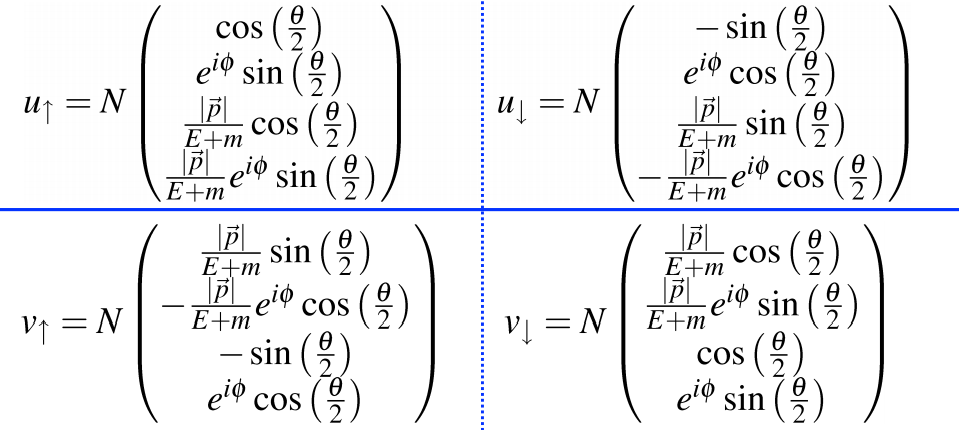
\includegraphics[width=0.6\linewidth]{espinores.png}
\end{center}
\caption{Espinores solución a la ecuación de Dirac y autoestados del operador helicidad.}
\label{espinores}
\end{figure}


\begin{figure}[!h]
\begin{center}
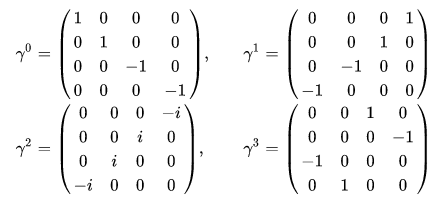
\includegraphics[width=0.6\linewidth]{matrices.png}
\end{center}
\caption{Matrices de Dirac.}
\label{matrices}
\end{figure}






\end{document}
